% Supporting mathematics, training/folding details, frozen evaluation protocols,
% deployment measurements and additional figures for the main manuscript.
\documentclass[10pt,twocolumn,letterpaper]{article}
\usepackage[margin=0.75in,columnsep=0.25in]{geometry}
\usepackage[T1]{fontenc}
\usepackage{mathptmx}
\usepackage{amsmath,amssymb}
\usepackage{graphicx,booktabs,array,tabularx}
\usepackage[font=small,labelfont=bf]{caption}
\usepackage{microtype}
\usepackage[hidelinks]{hyperref}
\urlstyle{rm}
\hypersetup{pdftitle={AEISU: Tensor Core-Accelerated Inverse Supersampling for Real-Time Game Upscaling -- Supplementary Material},
  pdfauthor={Charles Dale B. Gleason},
  pdfsubject={Inverse supersampling architecture, rendered-content evaluation, and output-head ablation}}
\setlength{\parindent}{1em}
\setlength{\parskip}{0pt}
\setlength{\textfloatsep}{11pt plus 2pt minus 2pt}
\setlength{\floatsep}{10pt plus 2pt minus 2pt}
\setlength{\abovedisplayskip}{6pt plus 2pt minus 1pt}
\setlength{\belowdisplayskip}{6pt plus 2pt minus 1pt}
\setlength{\emergencystretch}{1.2em}
\clubpenalty=10000
\widowpenalty=10000
\brokenpenalty=10000
\renewcommand{\topfraction}{0.9}
\renewcommand{\textfraction}{0.07}
\renewcommand{\floatpagefraction}{0.8}
\renewcommand{\dbltopfraction}{0.9}
\renewcommand{\dblfloatpagefraction}{0.55}
\setcounter{dbltopnumber}{3}
\newcommand{\model}{AEISU}
\newcommand{\R}{\mathbb{R}}
\newcommand{\A}{\mathcal{A}}
\newcolumntype{Y}{>{\raggedright\arraybackslash}X}
\renewcommand{\thesection}{S\arabic{section}}
\renewcommand{\thetable}{S\arabic{table}}
\renewcommand{\thefigure}{S\arabic{figure}}
\renewcommand{\theequation}{S\arabic{equation}}
\begin{document}
\raggedbottom
\twocolumn[{\begin{center}
{\Large\bfseries AEISU: Tensor Core-Accelerated Inverse Supersampling\\[2pt]
for Real-Time Game Upscaling\par}
\smallskip{\normalsize\bfseries Supplementary Material}\par
\smallskip{\small Charles Dale B. Gleason --- Independent Researcher}\par
\smallskip{\small Draft, 21 October 2026.}\par
{\scriptsize Copyright 2026 Charles Dale B. Gleason. \href{https://creativecommons.org/licenses/by/4.0/}{CC BY 4.0}; third-party imagery excluded.}\par
\end{center}\vspace{8pt}}]
\section{Analysis Stencils and Phases}
\label{app:stencils}
Each directional analysis operator is the cross-correlation of $y$ with a learned zero-sum difference stencil.
Writing the three parameters separately for each operator gives
\begin{align}
 D_x&=\begin{bmatrix}-a&0&a\\-b&0&b\\-c&0&c\end{bmatrix},&
 D_y&=\begin{bmatrix}-d&-e&-f\\0&0&0\\d&e&f\end{bmatrix},\\
 D_{45}&=\begin{bmatrix}-g&-h&0\\-i&0&i\\0&h&g\end{bmatrix},&
 D_{135}&=\begin{bmatrix}0&k&j\\-l&0&l\\-j&-k&0\end{bmatrix}.
 \label{eq:stencils}
\end{align}
The horizontal and vertical initial triplets are $(1/8,1/4,1/8)$; the two diagonal triplets are $(1/4,1/8,1/8)$.
Their zero sums follow from the difference construction, independently of the learned values.

Input-site parity uses $\rho=2(i\bmod2)+(j\bmod2)$.
Output phases are ordered top-left, top-right, bottom-left, bottom-right, corresponding to $(0,0),(0,1),(1,0),(1,1)$.
The coefficient tensor is parity-major: each of its four groups stores the sixteen coefficients of one LR site.
All output phases for that LR site reuse the same sixteen coefficients.

For the bilinear base initialization, the top-left output phase samples at $(-1/4,-1/4)$ relative to the source center.
The other phases use $(-1/4,+1/4)$, $(+1/4,-1/4)$, and $(+1/4,+1/4)$ in row--column order.
The four nonzero weights are products from $\{1/4,3/4\}$, giving $1/16$, $3/16$, and $9/16$ at their corresponding taps.
The learned deployed base can subsequently use the entire $5\times5$ support.

\section{Coefficient Perturbation Bound}
\label{app:bound}
Consider coefficient perturbations $\Delta a_k$ at a fixed site and phase, holding $L$, $B$, and $K$ fixed.
Using the main paper's RGB reconstruction definition,
\begin{equation}
 \Delta\widehat T_c=
   \sum_k\Delta a_k\sum_\delta K_{k,\phi}[\delta]\,
                                   L_c[\pi(p+\delta)].
\end{equation}
Zero DC allows subtraction of any constant $\mu_c$ inside the inner sum.
Let $r_c$ be the maximum minus minimum of the local channel samples, and choose $\mu_c$ to be their midpoint.
Then
\begin{equation}
 |\Delta\widehat T_c|
 \leq\frac{r_c}{2}\sum_k|\Delta a_k|\,\|K_{k,\phi}\|_1
 \leq\frac{\lambda r_c}{2}\|\Delta a\|_1.
 \label{eq:bound}
\end{equation}
Coefficient perturbations thus have less influence where the source neighborhood has a small channel range.
The coefficient clamp $g$ is 1-Lipschitz, so $|g(t+\Delta t)-g(t)|\leq|\Delta t|$.
This fixed-input, fixed-filter bound complements the complete-model quantization measurements in the main paper.


\section{Training and Kernel-space Folding}
\label{sec:training-folding}
The training set contains 635 Honkai: Star Rail frames and 65 Red Dead Redemption 2 frames selected from 8K capture banks by a pixel-diversity heuristic.
Recovered master-file mappings establish the two-source composition and retain the same 700 training targets.
For the UI-free Star Rail recordings, available OBS settings specify hardware NVENC AV1, Matroska recording, the high-quality recording option, I010 10-bit 4:2:0, sRGB, and full range.
These are compressed, perceptually encoded captures; the same recording settings are not established for the Red Dead Redemption 2 source bank.
The historical record does not recover exact rate control, all rendering/temporal settings, extraction color conversion, or complete scene-level membership.
The epoch-1000 final checkpoint was selected without internal validation.
The head-comparison validation images serve as visual diagnostics rather than checkpoint-selection data.

Checkpoint metadata and TensorBoard logs document the main paper's optimization recipe, the 1,000-epoch primary run, and the separate 100-epoch head studies.
The following subsection specifies reconstruction-gradient sampling.

\subsection{Reconstruction backward and sampling}
The custom kernel evaluates the full cropped RGB MSE and computes coefficient derivatives at every reconstructed LR site.
Spatial subsampling applies to the global base and adaptive-bank gradients, not to the reported loss or the coefficient-gradient field.
One LR site is selected per $16\times16$ block at offset $(r_y,r_x)$ supplied through the sampling-phase argument.
Its base and bank gradient contributions are multiplied by $16^2=256$ before reduction; all four output phases and RGB channels contribute at that site.
The reconstruction gradient then propagates through the zero-DC/$\ell_1$ projection and training-time parameterization.
The Area and Bicubic checkpoints, core controls and no-clamp control all use fixed offset $(r_y,r_x)=(0,0)$.
The residual and depth-to-space heads instead use dense autograd.

\subsection{Kernel-space folding maps}
Training assembles effective weights before convolution or reconstruction; it does not execute the alternate coordinates as separate image-sized branches.
For a convolution, let $\mathcal E$ embed a center, row, or column kernel in its deployed support.
The effective weight is
\begin{align}
 W_{\rm eff}={}&W_0+\mathcal E(U_1V_1+U_2V_2+D)\\
 &+\mathcal E(C)+\mathcal E(R)+\mathcal E(Q)
   +U_sV_s+\sum_t G_t\Psi_t+W_{\rm dw}.
\end{align}
The two center factorizations have ranks 8 and 16, capped by channel dimensions; $D$ is a diagonal channel route for square transforms.
The second line applies to $3\times3$ layers: $C$, $R$, and $Q$ are center, horizontal, and vertical coordinates; the spatial factorization has rank 8; six fixed directional templates $\Psi_t$ have learned channel-pair gains $G_t$; and $W_{\rm dw}$ is a per-channel spatial route when channel counts match.
The bias is unchanged.
Export stores $W_{\rm eff}$ and discards the alternate coordinates.

The analysis color matrix folds as $M=M_0+\operatorname{diag}(d)+UV$ with rank-two factors.
The luma mixture adds learned gains on BT.709 and uniform RGB vectors; each directional stencil adds learned gains on its initialization vector and $(0.5,-1,0.5)$.
These sums yield the 24 deployed analysis parameters.

For each phase, the base folds as
\begin{equation}
 B_\phi=B^0_\phi+\sum_{j=1}^{4}s_jB^j_\phi
                    +\mathcal R_\phi,
\end{equation}
where $\mathcal R_\phi$ combines centered $3\times3$, $1\times5$, $5\times1$, $1\times3$, $3\times1$, and $1\times1$ coordinates, two diagonals, 16 outer-ring taps, two separable factors, and eight fixed-template gains within the same $5\times5$ support.
The temporary bank uses the corresponding structured coordinates plus two dense $5\times5$ terms to form 64 four-phase kernels $F_{m,\phi}$.
With learned $A\in\R^{64\times16}$, its folded raw components are
\begin{equation}
 D_{k,\phi}=D^0_{k,\phi}+\sum_{m=0}^{63}A_{m,k}F_{m,\phi}.
\end{equation}
Zero-DC/$\ell_1$ projection is applied after this sum, producing the sixteen deployed effective components.

\section{Evaluation Protocols and Additional Results}
\label{sec:suppstats}
The expanded suite contains 39,000 reconstructions (13 methods, five conditions, 600 pairs) and 10,800 fixed-blur outputs.
The benchmark archive retains inputs, unchanged Native targets, float32 reconstructions, RGB8 previews, per-image scores, selection records, implementation hashes, and analysis source.

\subsection{Frozen model and implementation identities}
Table~\ref{tab:checkpoint-identities} identifies the seven learned checkpoints used in the expanded suite~\cite{conde2023repnet,zamfir2023rt4ksr,berger2023quicksrnet,wan2024span,liang2021swinir}.
Digest prefixes distinguish these files; \textnormal{research/quality/benchmark\_assets.json} in the companion repository contains full SHA-256 digests and available implementation records.
The tested SwinIR checkpoint is the lightweight DIV2K $2\times$ model, and SPAN uses 48 channels.
QuickSRNet uses the standard AIMET Model Zoo checkpoints and source revision \textnormal{1bd2bf5b17cd}.
Released neural models execute full-frame FP16 in channels-last PyTorch; SPAN and RT4KSR are deploy-folded, and SwinIR uses a shared attention-mask cache with mask dtype matched to FP16 logits.
The adaptive model uses its folded epoch-1000 checkpoint through the mixed native artifact.

The bicubic output baseline is PyTorch FP32 interpolation with \textnormal{align\_corners=False}, followed by clipping to $[0,1]$; it is distinct from the Pillow antialiased input degradation.
The main suite uses Native color at both resolutions: non-jittered, zero mipmap bias, with source AA and frame-blurring postprocessing disabled~\cite{mercier2023qrisp}.
The separate 60-frame head study uses AbandonedSchool's Enhanced targets, produced by downsampling 2160p MSAA$\times8$ renders to 1080p; it does not share the expanded study's Native targets.
Bilinear, EASU, EASU+RCAS, NIS, and SGSR1 use the frozen FP32 spatial-shader executable.
RCAS uses 0.2 stops; NIS uses sharpness zero.
AA sources are pinned to SMAA revision \textnormal{71c806a838bd} and the FXAA 3.11 header preserved in Intel CMAA2 revision \textnormal{071c6b085755}; settings are given in the main paper~\cite{jimenez2012smaa,lottes2011fxaa311}.
Implementation and shader hashes accompany the checkpoint records.
Compact records, source, and AEISU weights are provided in the \href{https://github.com/AELabs42/AEISU}{companion repository}.
The included Windows demo source uses the same mixed FP8/FP16 model; its comparison toggles and capture/presentation path are outside the benchmark harness. Prebuilt application binaries are not part of this source release.
\begin{table*}[t]
\centering\small
\caption{Learned checkpoint identities in the expanded QRISP suite. All checkpoints are $2\times$. SHA-256 prefixes are shown; full digests and implementation records are in \textnormal{benchmark\_assets.json}.}
\label{tab:checkpoint-identities}
\begin{tabularx}{\textwidth}{lYl}
\toprule
Method & Checkpoint filename & SHA-256 prefix\\
\midrule
AEISU mixed & {\footnotesize\textnormal{aif\_\allowbreak{}reparam\_\allowbreak{}aggressive64\_\allowbreak{}parallel32x4\_\allowbreak{}ep1000\_\allowbreak{}folded\_\allowbreak{}production.\allowbreak{}pt}} & {\footnotesize\textnormal{d0208712e0d5}} \\
RepNet & {\footnotesize\textnormal{repnet\_\allowbreak{}x2.\allowbreak{}pth}} & {\footnotesize\textnormal{27c898894589}} \\
RT4KSR & {\footnotesize\textnormal{rt4ksr\_\allowbreak{}x2.\allowbreak{}pth}} & {\footnotesize\textnormal{9ec750009284}} \\
QuickSRNet Small & {\footnotesize\textnormal{quicksrnet\_\allowbreak{}small\_\allowbreak{}2x\_\allowbreak{}checkpoint\_\allowbreak{}float32.\allowbreak{}pth.\allowbreak{}tar}} & {\footnotesize\textnormal{d95d70f1d236}} \\
QuickSRNet Medium & {\footnotesize\textnormal{quicksrnet\_\allowbreak{}medium\_\allowbreak{}2x\_\allowbreak{}checkpoint\_\allowbreak{}float32.\allowbreak{}pth.\allowbreak{}tar}} & {\footnotesize\textnormal{a0d176b40a64}} \\
SPAN & {\footnotesize\textnormal{spanx2\_\allowbreak{}ch48.\allowbreak{}pth}} & {\footnotesize\textnormal{561fd5cf419a}} \\
SwinIR-Light & {\footnotesize\textnormal{002\_\allowbreak{}lightweightSR\_\allowbreak{}DIV2K\_\allowbreak{}s64w8\_\allowbreak{}SwinIR-\allowbreak{}S\_\allowbreak{}x2.\allowbreak{}pth}} & {\footnotesize\textnormal{193b229909ca}} \\
\bottomrule
\end{tabularx}
\end{table*}

\subsection{Area-resolve agreement and frame selection}
For each supplied Native pair, form $R=\A_2(T)$ in float64 without intermediate uint8 rounding.
The selection score is
\begin{equation}
 e(L,T)=\frac{1}{|\Omega_4|}\sum_{p\in\Omega_4}
       \big(Y(L)[p]-Y(R)[p]\big)^2,
\end{equation}
where $Y$ is the encoded BT.601 conversion used in the main paper~\cite{basicsrmetrics} and $\Omega_4$ excludes four pixels on each side of the LR grid.
Pairs are ordered within each environment by increasing $e$, breaking ties lexicographically by source identity.
The lowest quarter is the most-agreement stratum, the highest quarter is the least-agreement stratum, and the middle half is the middle stratum.
The ranking matches the area-control operator and responds to texture, aliasing, alignment, and brightness as well as rendering differences.

Forty frames are selected per stratum.
For slot $j=0,\ldots,39$ in a stratum of size $n$, the candidate index is $\lfloor(j+0.5)n/40\rfloor$.
Candidates are searched in increasing distance from that index, breaking ties toward the lower index.
Previously selected identities are excluded.
Within a source sequence, the first pass requires an absolute frame-index separation of at least two from every already selected frame in the environment; a second pass permits separation one if necessary.
The spacing pass used for each identity is retained in the manifest.
This spacing guard reduces adjacent-frame selection; statistical resampling still uses source-sequence clusters.
The available pool contains 2,460 Native pairs; the frozen sample contains 600.

\subsection{Paired uncertainty}
We use 50,000 hierarchical bootstrap draws with seed 2026100402.
Each draw samples five environments with replacement and one source-sequence resample per named environment, weighting its sampled frames equally and retaining joint method/condition pairing.
Repeated selections of an environment share that inner resample, so these are coupled environment/sequence-weight bands rather than an independent inner resample for each selected occurrence; the edge and ablation analyses use the same coupling.
For each contrast, nominal intervals are the 2.5th/97.5th percentiles.
The simultaneous critical value is the 95th percentile of the maximum absolute standardized bootstrap deviation across the named family.
Bands equal the observed effect plus/minus this critical value times its bootstrap standard deviation.
The resulting bands use an approximate max-standardized-deviation bootstrap.

Four separate families contain 180 adaptive-versus-baseline contrasts, 30 within-adaptive input contrasts, 54 blur contrasts, and 138 cross-model/degradation interactions.
The last family contains eight comparator pairs on five conditions/three metrics and six area-to-bicubic relative-response contrasts on three metrics.
Multiplicity adjustment applies within each family.
With only five environments, even an exact two-sided environment sign-flip test has minimum attainable $p=2/32=0.0625$.
The bands are exploratory, with no specified equivalence margin.
As in the main text, inferential comparisons use bands excluding zero, while point estimates are identified as means.

\begin{table*}[t]
\centering\footnotesize
\setlength{\tabcolsep}{3pt}
\caption{Selected environment effects and leave-one-environment-out (LOO) sensitivity. All differences are AEISU minus the named comparator. PSNR is in dB (positive favors AEISU); LPIPS is unscaled (negative favors AEISU). AS: AbandonedSchool; BN: ScifiBaseNightStartStop; SF: ScifiFacility; SP: SeaPort; ST: SunTempleBush. These descriptive values do not assume calibrated small-sample confidence coverage.}
\label{tab:environment-sensitivity}
\begin{tabular}{llrrrrrrl}
\toprule
Condition / comparator & Metric & AS & BN & SF & SP & ST & Mean & LOO range\\
\midrule
Area / QuickSRNet S & PSNR & $+0.920$ & $+1.314$ & $+1.554$ & $+1.017$ & $+0.750$ & $+1.111$ & $[+1.000,+1.201]$\\
Area / SwinIR-Light & LPIPS & $+0.05175$ & $+0.01377$ & $+0.00331$ & $+0.02190$ & $+0.07852$ & $+0.03385$ & $[+0.02268,+0.04149]$\\
Native / EASU & PSNR & $-0.329$ & $-0.740$ & $-0.822$ & $-0.596$ & $-0.731$ & $-0.644$ & $[-0.722,-0.599]$\\
Native / EASU+RCAS & LPIPS & $+0.00173$ & $-0.00870$ & $-0.00932$ & $+0.00185$ & $-0.00812$ & $-0.00451$ & $[-0.00610,-0.00331]$\\
\bottomrule
\end{tabular}
\end{table*}

Table~\ref{tab:environment-sensitivity} shows selected environment means and leave-one-environment-out ranges alongside the exploratory intervals.
The Area PSNR gain over QuickSRNet Small and Native PSNR deficit to EASU retain their directions in all five environments; the small Native LPIPS lead over RCAS changes sign between environments.

The statistical record retains all contrasts, environment effects, leave-one-environment-out ranges, intervals, bands, and paired frame win fractions.
Y/RGB aggregate PSNR/SSIM comparison directions agree in all 120 adaptive-versus-baseline checks.
Frame fractions are descriptive; environments, not individual frames, are the top-level resampling units.

\subsection{Area-resolve agreement and texture}
\begin{table}[h]
\centering\small
\caption{Area-resolve agreement strata. These are descriptive sample averages, not isolated rendering-mismatch effects.}
\begin{tabular}{lrrr}
\toprule
Stratum & LR Y variance & Gradient energy & Pair Y MSE\\
\midrule
Most &0.02395&0.00593&0.000725\\
Middle &0.02917&0.01016&0.001369\\
Least &0.03284&0.01500&0.002147\\
\bottomrule
\end{tabular}
\end{table}
Some extreme strata have sparse sequence support.
AbandonedSchool's most/least strata each contain one sequence; SeaPort has one sequence in every stratum.
Joint cluster resampling can omit a stratum entirely.
Stratum results therefore use descriptive effects and leave-one-environment-out sensitivity.
The agreement score measures pair differences without identifying their cause.

\subsection{Numerical reproduction audit}
Hashes were checked for all 39,000 main PNG/NPZ pairs, and metrics were independently reproduced for 166 saved predictions spanning every main and blur configuration.
Maximum discrepancies were $7.11\times10^{-15}$ for distortion metrics and $6.23\times10^{-6}$ for LPIPS.
Identical-image batch/layout and FP64 controls attributed the LPIPS discrepancy to execution arithmetic, within an absolute tolerance of $10^{-5}$.
Sampling identities and diagnostics are recorded in \textnormal{verification\_v3.json}.

\subsection{Core architecture controls}
\label{sec:core-controls}
The original 100-epoch adaptive-head checkpoint is compared with three independently trained controls: fixed identity RGB mixtures, BT.709 luma and directional stencils; a fixed bilinear base; and two dense $64$-channel core convolutions in place of the parallel branches.
All use 700 training pairs, seed 1234, 87,500 updates, batch 32, $512\times512$ HR crops, D4 augmentation, RGB MSE and cosine decay from $2\times10^{-3}$ to $10^{-6}$, with fixed-offset stride-16 base/bank gradients and fused reconstruction.

The checkpoints are folded on CPU in FP32 before common FP16 controller execution and fused FP32 reconstruction.
Original RGB, analysis constants, base and adaptive-bank constants remain FP32.
All models use the established symmetric alignment to multiples of 32, a replicate halo of at least 16 LR pixels, and cropping back to the exact image extent.
The 600 frozen pairs, five input conditions and unchanged Native targets are those in the main evaluation.
Outputs are clipped to $[0,1]$ before scoring; float32 arrays and original-color PNG previews are retained.

\begin{table*}[t]
\centering\scriptsize
\setlength{\tabcolsep}{2.5pt}
\caption{Core-control reconstruction quality on the frozen 600-pair QRISP sample. Each group reports Y PSNR (P), Y SSIM (S) and RGB LPIPS (L), with two HR border pixels cropped. All checkpoints use the common FP16-controller/FP32-reconstruction implementation, not the production mixed runtime.}
\label{tab:core-quality}
\begin{tabular}{l*{15}{r}}
\toprule
 & \multicolumn{3}{c}{Area} & \multicolumn{3}{c}{Bicubic} & \multicolumn{3}{c}{FXAA} & \multicolumn{3}{c}{SMAA} & \multicolumn{3}{c}{Native}\\
Control & P & S & L & P & S & L & P & S & L & P & S & L & P & S & L\\
\midrule
Reference &31.297&.91375&.11390&31.033&.90707&.15198&27.496&.84092&.19070&27.147&.85003&.17184&26.682&.84724&.16188\\
Fixed inputs &31.304&.91395&.11219&31.057&.90751&.15065&27.493&.84103&.19000&27.137&.84995&.17090&26.676&.84722&.16068\\
Fixed bilinear base &31.283&.91346&.11395&31.029&.90691&.15217&27.496&.84089&.19133&27.142&.84990&.17232&26.690&.84740&.16210\\
Dense $64\times2$ core &31.277&.91370&.11396&31.015&.90724&.15156&27.495&.84098&.19028&27.147&.84997&.17154&26.687&.84735&.16091\\
\bottomrule
\end{tabular}
\end{table*}

Paired environment/sequence bootstrap intervals use 3,000 resamples and a common family of 45 contrasts: three controls, five conditions and three primary metrics.
Fixed inputs improve all three Bicubic metrics: $+0.024$ dB PSNR, $+0.00044$ SSIM and $-0.00132$ LPIPS, but lower SMAA PSNR by $0.010$ dB.
The fixed base lowers Area and Bicubic SSIM and increases FXAA LPIPS; the dense core lowers Area PSNR by $0.020$ dB.
These are the contrasts whose simultaneous bands exclude zero; all remaining core-quality bands span zero.
The fixed analysis/base retain the reference's deployed operator shapes; the dense core matches bottleneck convolution MACs but not depth or channel connectivity.

\paragraph{RGB reconstruction check.}
Across the five conditions, the learned-analysis reference differs from the fixed-input control by $-0.023$ to $+0.010$ dB in mean RGB PSNR and by at most $0.00054$ in mean RGB SSIM.
The color mixtures guide coefficient prediction; reconstruction still reads the original RGB channels.

\paragraph{Coefficient-predictor FP8 stress.}
A separate Area-only stress test rounds every controller convolution's weights and inputs to E4M3, then evaluates dequantized convolutions with FP32 arithmetic.
Weight scales are per output channel; activation scales are per layer and tensor, using maxima from the same 24 fixed, centered $128\times128$ LR training crops for every model.
Biases, original RGB, analysis and reconstruction constants remain FP32, and no bias correction is applied.
Table~\ref{tab:core-quantization} reports absolute scores and within-model changes for this software rounding test, distinct from the native head study and the deployed stage-specific FP8/FP16 configuration.

\begin{table}[h]
\centering\small
\setlength{\tabcolsep}{3pt}
\caption{Area coefficient-predictor FP8 rounding stress on 600 pairs. Changes are FP8 stress minus each model's own FP16 result. Positive LPIPS change is degradation.}
\label{tab:core-quantization}
\begin{tabularx}{\columnwidth}{Yrrrr}
\toprule
Control & FP8 PSNR & $\Delta$PSNR & $\Delta$SSIM & $\Delta$LPIPS\\
\midrule
Reference &31.259&$-.03766$&$-.000953$&$-.000240$\\
Fixed inputs &31.251&$-.05284$&$-.000975$&$+.000618$\\
Fixed bilinear base &31.206&$-.07733$&$-.001516$&$+.003623$\\
Dense $64\times2$ core &31.202&$-.07510$&$-.001729$&$+.001848$\\
\bottomrule
\end{tabularx}
\end{table}

All four within-model PSNR and SSIM decreases exclude zero under a separate 12-contrast simultaneous-band family.
Only the fixed base's within-model LPIPS increase excludes zero.
A further nine-contrast family identifies three precision-change differences from the reference: an additional $0.00386$ LPIPS increase for the fixed base, and an additional $0.000775$ SSIM loss and $0.00209$ LPIPS increase for the dense core.

All 28,800 output files are present.
An independent check reproduced 48 first/last predictions spanning all 24 configurations, including array hashes and half-up PNG rounding; metric discrepancies were at most $7.11\times10^{-15}$ for distortion and $5.96\times10^{-8}$ for LPIPS.

\subsection{Coefficient-clamp control}
\label{sec:clamp-ablation}
The no-clamp checkpoint replaces the soft transfer with $g(t)=t$, leaving the learned analysis, parallel core, base and sixteen-component $5\times5$ bank unchanged.
It uses the same 700 Area pairs, seed 1234, 100 epochs, 87,500 updates, batch 32, $512\times512$ HR crops, D4 augmentation, RGB MSE and cosine decay from $2\times10^{-3}$ to $10^{-6}$.
Optimizer state and all 100 TensorBoard epoch records agree with the checkpoints and schedule.
Final training MSE is $1.14711\times10^{-4}$ with the clamp and $1.16643\times10^{-4}$ without it.
Both runs use fused training reconstruction and fixed-offset stride-16 base/bank gradients.

Both checkpoints are folded in CPU FP32 and use common FP16 controller execution, FP32 tiled reconstruction, the established alignment/halo convention, and clipping to $[0,1]$ before scoring.
All 600 frozen pairs and five input conditions are retained.
Tiled reconstruction evaluates each checkpoint's own coefficient transfer.
The reference's tiled/fused preflight discrepancy is below $5.4\times10^{-7}$.

\begin{table*}[t]
\centering\scriptsize
\setlength{\tabcolsep}{2.5pt}
\caption{Coefficient-clamp control on 600 QRISP pairs per condition. P: Y PSNR; S: Y SSIM; L: RGB LPIPS, with two HR border pixels cropped. Both 100-epoch checkpoints use common FP16-controller/FP32 tiled reconstruction.}
\label{tab:clamp-quality}
\begin{tabular}{l*{15}{r}}
\toprule
 & \multicolumn{3}{c}{Area} & \multicolumn{3}{c}{Bicubic} & \multicolumn{3}{c}{FXAA} & \multicolumn{3}{c}{SMAA} & \multicolumn{3}{c}{Native}\\
Transfer & P & S & L & P & S & L & P & S & L & P & S & L & P & S & L\\
\midrule
Soft clamp &31.297&.91375&.11390&31.033&.90707&.15198&27.496&.84092&.19070&27.147&.85003&.17184&26.682&.84724&.16188\\
Identity &31.253&.91331&.11513&31.005&.90683&.15297&27.498&.84098&.19149&27.153&.85010&.17281&26.695&.84758&.16315\\
\bottomrule
\end{tabular}
\end{table*}

Paired environment/sequence bootstrap bands use 3,000 resamples, seed 20261010, and a 15-contrast family for the five-condition quality comparison.
No-clamp minus clamped Area PSNR is $-0.0436$ dB (simultaneous band $[-0.0725,-0.0147]$); Bicubic PSNR is $-0.0277$ dB ($[-0.0481,-0.0073]$).
Area and Bicubic SSIM also decrease, while SMAA PSNR increases by $0.0060$ dB.
LPIPS increases by $0.00099$ on Bicubic and $0.00079$ on FXAA.
The remaining quality contrasts have simultaneous bands spanning zero.

\paragraph{Precision sensitivity.}
The Area-only E4M3 rounding protocol and 24 centered training-calibration crops match the core controls: per-output-channel weight scales, per-layer activation scales, dequantized FP32 convolutions, and FP32 biases, analysis and reconstruction constants.
Table~\ref{tab:clamp-quantization} separates absolute quality from within-model precision changes.

\begin{table}[t]
\centering\small
\setlength{\tabcolsep}{3pt}
\caption{Coefficient-clamp Area FP8 rounding stress. Changes are relative to each checkpoint's FP16 result, not the production mixed runtime.}
\label{tab:clamp-quantization}
\begin{tabularx}{\columnwidth}{Yrrrr}
\toprule
Transfer & FP8 PSNR & $\Delta$PSNR & $\Delta$SSIM & $\Delta$LPIPS\\
\midrule
Soft clamp &31.259&$-.03766$&$-.000953$&$-.000240$\\
Identity &31.184&$-.06932$&$-.001168$&$+.001158$\\
\bottomrule
\end{tabularx}
\end{table}

The six-contrast family identifies PSNR/SSIM losses in both checkpoints and LPIPS degradation in the no-clamp checkpoint.
Two of the three precision-change contrasts separate from the reference: removing the clamp adds $0.0317$ dB PSNR loss (band $[0.0146,0.0487]$) and a $0.00140$ LPIPS increase (band $[0.00014,0.00265]$).

\paragraph{Coefficient magnitudes.}
Statistics exclude the padded halo and distinguish raw predictions $\widetilde a$ from applied coefficients $a$.
On Area, mean per-image raw RMS is $1.029$ with the clamp versus $2.633$ without; mean per-image sampled absolute 99th percentiles are $3.103$ and $8.683$, using 4,096 deterministic samples per image.
The fractions of raw magnitudes above 2 are $5.07\%$ and $35.72\%$.
The soft branch compresses predictions above 2; only about $1.95\times10^{-7}$ of the reference's raw coefficients exceed 12, where the applied cap is reached.
Applied maxima on Area are $2.5$ and $63.906$, respectively.
Raw maxima on Area are $19.188$ and $63.906$; across all five conditions, they reach $23.578$ with the clamp and $86.938$ without it.
The no-clamp checkpoint therefore has both larger typical raw magnitudes and larger extremes.

All 7,200 float32 reconstructions and PNG previews were saved.
Coverage checks confirm all 14,400 files; an independent 24-output first/last sample spans every configuration and reproduces hashes, decoding, preview rounding and metrics, with discrepancies below $7.11\times10^{-15}$ for distortion and $7.28\times10^{-6}$ for LPIPS.

\subsection{Training-degradation comparison}
\label{sec:training-degradation}
A second 1,000-epoch checkpoint uses MATLAB-style antialiased bicubic inputs downscaled directly from the original 8K masters to 1080p, retaining the area-trained model's 700 4K targets.
For a master $S$, these pairs use $T=\A_2(S)$ and $L=\mathcal B_4(S)$, where $\mathcal B_s$ is bicubic reduction by $s$.
This common-master chain is generally different from $L=\mathcal B_2(T)$, the target-derived bicubic construction used by the benchmark.
Both checkpoints have 875,000 updates, seed 1234, batch 32, $512\times512$ HR crops, D4, RGB MSE and cosine decay from $2\times10^{-3}$ to $10^{-6}$, with fixed-offset stride-16 base/bank gradients and fused reconstruction.
Final training MSE is $1.13810\times10^{-4}$ for Area and $1.08882\times10^{-4}$ for Bicubic; these losses use different input distributions.
Evaluation uses the core controls' common FP16 controller/FP32 reconstruction, padding, 600 pairs, and metrics.
All methods receive the same Pillow-antialiased Bicubic inputs, including released models trained with MATLAB-style resizing; the two bicubic implementations are not identical.

\begin{table*}[t]
\centering\footnotesize
\setlength{\tabcolsep}{2.5pt}
\caption{Training-degradation comparison on 600 QRISP pairs per input condition. P: Y PSNR; S: Y SSIM; L: RGB LPIPS. Both 1,000-epoch checkpoints use common FP16 evaluation; these are separate from the mixed-production scores in the main comparison.}
\label{tab:training-degradation}
\begin{tabular}{l*{15}{r}}
\toprule
 & \multicolumn{3}{c}{Area} & \multicolumn{3}{c}{Bicubic} & \multicolumn{3}{c}{FXAA} & \multicolumn{3}{c}{SMAA} & \multicolumn{3}{c}{Native}\\
Training & P & S & L & P & S & L & P & S & L & P & S & L & P & S & L\\
\midrule
Area &31.346&.91446&.11238&31.060&.90776&.15146&27.496&.84111&.19015&27.141&.85010&.17107&26.674&.84732&.16104\\
Bicubic &30.606&.90875&.09864&31.725&.91664&.12067&27.348&.83856&.17522&26.766&.84341&.16130&25.956&.83386&.16355\\
\bottomrule
\end{tabular}
\end{table*}

With 3,000 paired environment/sequence resamples and a simultaneous family of 15 contrasts, Bicubic training raises Bicubic PSNR by $0.665$ dB (band $[0.330,1.001]$), but lowers Area PSNR by $0.740$ dB and Native PSNR by $0.718$ dB.
PSNR and SSIM favor Area training on Area, FXAA, SMAA and Native, and Bicubic training on Bicubic.
Bicubic training lowers LPIPS on Area by $0.01375$, Bicubic by $0.03079$ and FXAA by $0.01493$.
Only the mean SMAA LPIPS decrease and Native increase have bands spanning zero in this family.
The Bicubic-minus-Area input interaction is $+1.405$ dB PSNR (band $[0.965,1.845]$) under a separate three-metric family.
The Bicubic-trained checkpoint still has lower mean Bicubic PSNR and higher LPIPS than SPAN and SwinIR-Light in the main comparison.

\subsection{Target-selected isolated-edge profiles}
\label{sec:isolated-edges}
The archived-output diagnostic selects coherent edges with approximately flat flanks from the unchanged HR targets only.
A fixed target-gradient grid, seed 20261004, and cap of 512 profiles/frame yield 40,517 profiles in 570 frames; the other 30 frames are excluded identically for all methods.
All thirteen methods and five input conditions use the same positions and edge normals.
Profiles span $\pm12$ HR pixels at half-pixel spacing and average three parallel tangent samples.
Plateau medians use the outer 8--12 pixels.
Eligibility requires target contrast at least $0.08$, gradient at least $0.015$, coherence at least $0.85$, plateau spread at most $6\%$ of target contrast, and limited target oscillation.
The source protocol and region coordinates retain the complete selection thresholds.

Bright/dark excursions are departures from each prediction's own plateau envelope, after subtracting the target's corresponding excursion and normalizing by target contrast.
Ringing is excess non-monotonic total variation over the target, divided by twice target contrast.
Transition width uses the prediction's own plateau-normalized 10--90\% crossings, and retained contrast is its plateau difference divided by target contrast.
Frame means are equally weighted within each environment, then the five environments equally weighted.
The paired environment/sequence bootstrap uses 10,000 draws and simultaneous bands for twelve comparators times three diagnostics separately within each input condition.
The resampling units are evaluation environments and source sequences.

\begin{table*}[t]
\centering\footnotesize
\setlength{\tabcolsep}{4pt}
\caption{Target-selected isolated-edge diagnostic on 570 frames. B: bright excursion; R: excess profile ringing (both percentages of target edge contrast, lower is better); W: 10--90\% transition width in HR pixels. Means weight frames within environments, then environments equally. These are custom profile measurements, not whole-image quality scores.}
\label{tab:edge-profiles}
\begin{tabular}{l*{9}{r}}
\toprule
 & \multicolumn{3}{c}{Area} & \multicolumn{3}{c}{Bicubic} & \multicolumn{3}{c}{Native}\\
\cmidrule(lr){2-4}\cmidrule(lr){5-7}\cmidrule(lr){8-10}
Method & B & R & W & B & R & W & B & R & W\\
\midrule
AEISU mixed & 0.683 & 1.869 & 3.042 & 1.568 & 2.765 & 3.178 & 1.245 & 4.208 & 2.946\\
Bilinear & 0.079 & 0.764 & 4.367 & 0.583 & 1.337 & 4.359 & 0.118 & 0.777 & 4.100\\
Bicubic & 2.428 & 4.383 & 3.810 & 2.778 & 5.118 & 3.807 & 3.842 & 6.902 & 3.530\\
EASU & 0.108 & 0.582 & 3.613 & 1.529 & 2.617 & 3.584 & 0.203 & 0.820 & 3.433\\
EASU+RCAS & 2.215 & 4.415 & 3.333 & 4.088 & 7.791 & 3.337 & 2.556 & 5.158 & 3.139\\
NIS & 1.900 & 4.811 & 3.805 & 2.180 & 5.008 & 3.818 & 3.653 & 8.843 & 3.498\\
SGSR1 & 0.286 & 0.835 & 3.128 & 1.668 & 2.745 & 3.077 & 0.407 & 1.112 & 3.000\\
RepNet & 3.923 & 11.306 & 3.313 & 3.243 & 8.665 & 3.332 & 7.637 & 19.666 & 3.080\\
RT4KSR & 3.525 & 12.543 & 3.298 & 2.832 & 9.127 & 3.328 & 7.021 & 21.449 & 3.043\\
QuickSRNet S & 3.223 & 8.834 & 3.104 & 1.692 & 4.517 & 3.107 & 6.656 & 16.088 & 2.892\\
QuickSRNet M & 2.816 & 7.969 & 3.086 & 1.283 & 3.068 & 3.108 & 6.202 & 15.144 & 2.849\\
SPAN & 2.954 & 8.333 & 3.128 & 0.976 & 1.997 & 3.073 & 8.337 & 31.214 & 3.068\\
SwinIR-Light & 3.161 & 8.016 & 3.101 & 0.930 & 2.002 & 3.070 & 7.226 & 16.729 & 2.853\\
\bottomrule
\end{tabular}
\end{table*}


On Area, AEISU has lower bright excursions and ringing than all six neural comparators.
Mean dark undershoot is also lower, with bands spanning zero.
AEISU's retained contrast is $1.0003$ and its transition width is $3.042$ pixels against the target's $2.995$ pixels; reduced excursions are not accompanied by broad edge smoothing.
Bilinear, EASU, and SGSR1 nevertheless have lower bright excursions and ringing than AEISU.
The effect reverses on Bicubic: SPAN and SwinIR-Light have lower bright/dark excursions and ringing, and QuickSRNet Medium has lower bright/dark excursions.
AEISU retains lower ringing than all six neural comparators on FXAA and SMAA, although fewer bright-excursion contrasts separate under the bands.
On Native, AEISU has lower bright excursions and ringing than all six neural comparators; bilinear, EASU, and SGSR1 remain lower than AEISU.
Independently rendered inputs prevent interpreting every Native profile difference as a newly synthesized artifact.

This custom diagnostic passed synthetic sharp, blurred, shifted, constant, gain-biased, and known-ringing checks.
Width, contrast, and fidelity distinguish sharp, low-ringing edges from blurred or constant outputs, which can also have zero excursions.
The diagnostic covers post-clipping isolated-edge behavior within the fixed profile window; textured and multiple-edge regions are excluded.

\subsection{Saved-output smoothing and paired transfer controls}
\label{sec:saved-controls}
The Area extension applies the original Gaussian grid ($\sigma=0.5,1,2$ HR pixels, radius $\lceil3\sigma\rceil$, replicated borders) to saved float32 RGB predictions for AEISU and EASU.
It evaluates encoded-Y PSNR/SSIM on all 600 unchanged targets with the original two-HR-pixel crop and equal environment weighting.
Every unblurred distortion score was reproduced within $10^{-10}$ before smoothing.
This extension measures distortion only; the original Native/FXAA/SMAA LPIPS sweep is unchanged.
The paired transfer control subtracts each frame's Area AEISU-minus-EASU PSNR gap from its Native gap.
Nominal intervals use 10,000 paired environment/sequence draws, separately within each stratum.
The subtraction adjusts for each frame's observed Area comparator gap.

\begin{table}[t]
\centering\footnotesize
\caption{Gaussian smoothing change in Y PSNR (dB) on the unchanged target. Negative values indicate reduced fidelity.}
\label{tab:area-blur-control}
\begin{tabularx}{\columnwidth}{Yrrr}
\toprule
Input / method & $\sigma=.5$ & $\sigma=1$ & $\sigma=2$\\
\midrule
Area / AEISU & $-.393$ & $-2.436$ & $-4.776$\\
Area / EASU & $-.315$ & $-1.453$ & $-3.273$\\
Native / AEISU & $+.588$ & $+.646$ & $-.587$\\
Native / EASU & $+.085$ & $-.202$ & $-1.311$\\
\bottomrule
\end{tabularx}
\end{table}

All three Area settings lower SSIM as well: AEISU changes by $-0.00939$, $-0.06036$, and $-0.15399$; EASU by $-0.01044$, $-0.05057$, and $-0.12805$.
At $\sigma=1$, the AEISU Native-versus-Area PSNR response differs by $3.082$ dB.

\begin{table}[t]
\centering\footnotesize
\caption{Paired transfer gaps in Y PSNR (dB): AEISU minus EASU. D: Native gap minus Area gap; brackets show nominal 95\% environment/sequence bootstrap intervals.}
\label{tab:paired-transfer-gap}
\begin{tabularx}{\columnwidth}{Yrrr}
\toprule
Stratum & Native & Area & D [interval]\\
\midrule
All & $-.644$ & $+1.648$ & $-2.291$\\
 & & & $[-2.831,-1.756]$\\
Most agreement & $-.515$ & $+1.759$ & $-2.274$\\
 & & & $[-2.761,-1.812]$\\
Middle & $-.674$ & $+1.660$ & $-2.334$\\
 & & & $[-2.860,-1.790]$\\
Least agreement & $-.742$ & $+1.523$ & $-2.266$\\
 & & & $[-2.986,-1.608]$\\
\bottomrule
\end{tabularx}
\end{table}

The most-versus-least Native gap narrows alongside a nearly equal change in the Area gap, leaving close adjusted stratum means.
Agreement sorting therefore reflects common image difficulty as well as Native rendering differences.

\subsection{DIV2K training and classic bicubic evaluation}
\label{sec:classic-bicubic}
The separate natural-image checkpoint retains the deployed 115,996-parameter architecture and is trained from fresh initialization on exactly the 800 official DIV2K training HR/$2\times$ bicubic pairs.
Training uses seed 1234, batch 32, $512\times512$ HR crops with the established LR context, D4, RGB L1, AdamW and cosine decay from $2\times10^{-3}$ to $10^{-6}$ over 3,000 epochs.
The variable-sized DIV2K images yield 305 updates per epoch and 915,000 updates in total, versus 875,000 in the game-data runs.
Base/bank gradients use fixed stride 16 at offset $(0,0)$ with fused training reconstruction and BF16 AMP.
The final epoch has training L1 $1.55376\times10^{-2}$; no classic benchmark image is used for training or checkpoint selection.

Table~\ref{tab:div2k-training} retains the earlier fresh 1,000-epoch MSE run (305,000 updates) on the same 800 pairs.
The L1/3,000-epoch run improves mean PSNR and SSIM on all four sets; LPIPS improves on Urban100 but is slightly worse on Set5, Set14 and B100.
Because both loss and training duration change, their contributions are not separated by this comparison.

% Generated by tools/paper_figures/classic_bicubic_results.py.
\begin{table}[t]
\centering\small
\caption{DIV2K training comparison. MSE: 1,000 epochs/305,000 updates; L1: 3,000 epochs/915,000 updates. P: Y PSNR (dB); S: Y SSIM; L: RGB LPIPS. Both checkpoints use the same evaluation path.}
\label{tab:div2k-training}
\begin{tabular}{lrrr}
\toprule
Dataset / loss & P & S & L\\
\midrule
Set5 MSE &37.054&0.95709&0.05901\\
Set5 L1 &37.098&0.95741&0.06068\\
Set14 MSE &32.685&0.91055&0.10327\\
Set14 L1 &32.721&0.91098&0.10409\\
B100 MSE &31.608&0.89250&0.15268\\
B100 L1 &31.630&0.89269&0.15294\\
Urban100 MSE &30.304&0.90875&0.09031\\
Urban100 L1 &30.365&0.90969&0.08924\\
\bottomrule
\end{tabular}
\end{table}


The evaluation includes every image in Set5 (5), Set14 (14), BSD100/B100 (100) and Urban100 (100), with frozen input/target hashes.
All evaluated variants receive the same archived MATLAB-style antialiased bicubic $2\times$ LR images; odd HR dimensions are scale-modcropped without resampling.
The common metric implementation evaluates floating-point clipped RGB outputs, with BT.601 encoded-Y PSNR/SSIM and RGB LPIPS-AlexNet v0.1 after cropping two HR border pixels.
Scores are per-dataset image means, separate from the QRISP environment-bootstrap analysis.

The FP16 row uses the FP16 controller and FP32 reconstruction reference implementation.
The native mixed artifact folds the same checkpoint in FP32 and retains FP16 projection/refinement/head with FP8 internal stages.
Scales and bias corrections use 24 evenly spaced DIV2K training inputs with $128\times128$ LR crops and two scale-search passes; six other training inputs provide disjoint calibration checks, not model-held-out evaluation.
No classic benchmark image enters calibration.
The native path includes RGBA16F input/output storage.
Mixed deployment loses $0.007$--$0.019$ dB in dataset-mean Y PSNR and adds $0.00010$--$0.00095$ LPIPS; the largest per-image PSNR decrease is $0.151$ dB, with four images losing more than $0.1$ dB.

FSRCNN uses the released luminance checkpoint from \href{https://github.com/yjn870/FSRCNN-pytorch/blob/master/test.py}{FSRCNN-pytorch}: FP32 inference on BT.601 limited-range Y, with a PyTorch-bicubic RGB carrier supplying chroma.
All methods' Y and RGB scores are recomputed from their final RGB outputs, including clipping; the FSRCNN values therefore follow this RGB-output protocol rather than a separately rounded Y-only evaluation.
The remaining neural checkpoints and adapters are those in the QRISP comparison.
The archive retains the original 2,190 reconstructions and 219 outputs for each L1 precision variant (2,628 total), their PNG previews, model identities and per-image scores, with complete identity coverage and verified output hashes.
The L1 evaluations reuse the original comparator scores after checking identical source-image hashes and metric settings; eight saved outputs per L1 precision variant reproduce the recorded distortion and LPIPS values.
The main paper's classic-bicubic table reports quality for this checkpoint; the optimized mixed-runtime measurements use the original area-trained game checkpoint.

\section{Precision and Runtime Details}
\subsection{Numerical precision and calibration}
\label{sec:precision}
We measure numerical agreement with the FP32 output separately from reconstruction quality against HR targets.
The natural-image precision and output-head diagnostics use 219 HR images from Set5, Set14, B100, and Urban100.
Each image is cropped at its bottom/right edge to even dimensions, then aligned $2\times2$ cells are averaged and rounded to uint8 by $\lfloor(\mathrm{sum}+2)/4\rfloor$.
Evaluation uses encoded RGB divided by 255, clipped outputs, and full-image RGB/Y metrics; SSIM uses an $11\times11$ Gaussian window with $\sigma=1.5$, population moments, and valid interior~\cite{wang2004ssim}.
The FP32 reference disables TF32 and automatic mixed precision; native RGBA16F image storage introduces rounding in addition to arithmetic differences.
Calibration uses per-output-channel E4M3 weight error minimization/least-squares scaling, activation-scale coordinate descent against FP32 reconstructed RGB, and bias correction.
We use 24 training images and six separate calibration-validation images with $128\times128$ crops; benchmark images are not used for calibration.
Uniform FP8 uses FP8 operands throughout the controller and shares calibration with the mixed-precision configuration.

Across all images, mixed-to-FP32 PSNR averages 54.594 dB, with a minimum of 31.658 dB; FP16 remains above 68.154 dB on every image.
Mixed precision changes mean target RGB PSNR by $-0.0125$ dB relative to FP32.
The fifth percentile of the per-image target PSNR change is $-0.0426$ dB; nine images lose more than $0.05$ dB and three more than $0.1$ dB.
The largest loss and lowest numerical agreement both occur on Urban100's \textnormal{img011.png}, a high-contrast building facade with repeated narrow structures.
Its full-image target RGB PSNR decreases from $22.818$ to $22.339$ dB ($-0.479$ dB), and RGB SSIM decreases by $0.00377$.
The other two losses above $0.1$ dB are \textnormal{img096.png} ($0.170$ dB) and \textnormal{img062.png} ($0.133$ dB).

\subsection{Runtime and resource use}
\begin{table*}[t]
\centering\small
\caption{Common ordinary-PyTorch resident timing in ms, median (p95). Five trials, 20 warmup and 50 measured forwards; batch one, full frame, FP16, TF32 disabled, channels-last, cuDNN autotuning. Eager and CUDA graph (G) execution use the same operators. The final auxiliary row retains FP32 analysis and synthesis, unlike the uniform-FP16 rows.}
\label{tab:common-runtime}
\begin{tabularx}{\textwidth}{Yrrrr}
\toprule
 & 540p$\to$1080p E & 540p$\to$1080p G & 1080p$\to$4K E & 1080p$\to$4K G\\
\midrule
AEISU & 1.721 (1.761) & 1.588 (1.592) & 7.064 (7.082) & 6.905 (6.917)\\
QuickSRNet S & 0.326 (0.331) & 0.292 (0.294) & 1.860 (1.868) & 1.839 (1.842)\\
QuickSRNet M & 0.611 (0.617) & 0.554 (0.558) & 3.545 (3.554) & 3.505 (3.513)\\
RepNet & 0.173 (0.244) & 0.129 (0.130) & 0.535 (0.541) & 0.514 (0.517)\\
RT4KSR & 1.108 (1.263) & 0.509 (0.511) & 1.968 (2.241) & 1.719 (1.725)\\
SPAN & 5.922 (5.956) & 5.820 (5.846) & 30.996 (31.192) & 30.884 (31.032)\\
SwinIR-Light & 124.587 (124.876) & 123.529 (123.811) & 499.289 (499.491) & 498.413 (498.857)\\
AEISU (FP32 synthesis) & 2.770 (2.788) & 2.661 (2.664) & 13.172 (13.199) & 13.022 (13.050)\\
\bottomrule
\end{tabularx}
\end{table*}

Uniform FP8 latency increases from $0.488$ to $1.132$ ms between 1080p and 1440p input ($2.32\times$), exceeding the $1.78\times$ nominal pixel ratio ($1.745\times$ after the recorded padding).
Its detailed-event analysis/projection stage increases from $0.0511$ to $0.1679$ ms and coefficient head from $0.0346$ to $0.1632$ ms; refinement also increases from $0.1741$ to $0.3951$ ms.
Minimal-event trial ranges are narrow ($0.4869$--$0.4887$ and $1.1301$--$1.1345$ ms), reproducing the earlier session's nonlinear scaling in a fresh five-trial sweep.
The excess is localized to these stages; its hardware or library cause remains undetermined.
Detailed instrumentation changes execution overhead and is not substituted for minimal-event total latency.
The implementation uses SM120a-specific mixed kernels and uniform-FP8 cuDNN refinement, so pixel-count scaling alone is not a sufficient performance model.
\label{sec:timing}
Measurements use an RTX 5090; the harness records hardware state but does not change clock or power settings.
The native runtime uses driver 616.92, CUDA 13.4, and cuDNN 9.25; the independent Python reference uses PyTorch 2.11.0 with CUDA 13.0.
The resolution sweep uses 100 warmup iterations and 200 measured iterations per trial, with five trials per precision and resolution.
Median latency is the median of trial medians, and p95 is the median of within-trial p95 values.
The resolution-sweep results are reported in the main paper.

The interval begins after the external input fence wait and ends after reconstruction, before the output-ownership signal.
It includes analysis, controller execution, required layout/format conversions, and reconstruction, but excludes resource creation, graph construction, CPU submission, D3D readback, capture, and presentation.
Measurements use CUDA graphs, batch size one, and steady-state single-slot execution.
A fixed natural image is resized to each input shape for timing.
Runtime spatial padding includes a source halo and tile alignment: 1080p input is processed in a $1952\times1120$ source domain before cropping.
The common-runtime complexity table includes this controller border work; the nominal per-LR-pixel formula does not.
The repeated 1080p mixed p95 is $0.440$ ms, consistent with the earlier matched-deployment session's $0.439$ ms but not the historical sweep's $0.678$ ms.
The historical sweep remains separately archived; the cause of its larger tail latency is unknown.


\begin{table*}[t]
\centering\small
\caption{Stage times for 1080p input ($\mu$s), measured with CUDA event instrumentation. Entries combine medians of constituent operations. Instrumentation changes timing relative to the unprofiled resolution sweep.}
\label{tab:stage-profile}
\begin{tabular}{lrrrl}
\toprule
Logical stage & FP8 & FP16 & Mixed & Interpretation\\
\midrule
Analysis + projection &51.104&59.440&42.912&Analysis and first learned projection\\
Compression + four core stages &87.744&594.032&97.680&Includes required unshuffle/conversion\\
Expansion + shuffle + skip &40.960&79.872&28.864&Mixed fuses shuffle and skip-add\\
Refinement + coefficient head &208.672&138.112&137.216&FP16/mixed fuse the two convolutions\\
RGB reconstruction &127.040&125.600&126.272&Conventional CUDA; shared reconstruction role\\
\bottomrule
\end{tabular}
\end{table*}

The stage comparison in Table~\ref{tab:stage-profile} motivates mixed precision: the FP8 core is substantially faster than its FP16 counterpart, whereas the fused FP16 refinement/head is faster than the FP8 route.
The gain reflects both numerical precision and the fusion and conversion choices of each route.
The controller paths use MMA/WMMA instructions with FP32 accumulation.
RGB reconstruction uses conventional CUDA arithmetic.

\subsection{Secondary conventional-CUDA deployment}
\label{sec:shader-deployment}
The secondary deployment uses the same folded checkpoint, with FP16 projection/refinement/head and INT8 compression, parallel-core, and expansion convolutions.
Packed DP4A instructions accumulate integer convolutions in INT32; paired half arithmetic handles FP16 convolutions.
Analysis and RGB reconstruction remain FP32.
Symmetric per-output-channel weight quantization and existing FP8 activation ranges mapped to signed INT8 require no retraining.
The layer policy follows measured fused-group timings.

Seven kernels fuse analysis/projection, expansion/shuffle/skip addition, and refinement/head; adjacent core stages retain intermediates in shared memory, and reconstruction shares RGB neighborhoods across output phases.

Table~\ref{tab:shader-deployment} compares the two deployments in the same timing session on RTX 5090.
Each resolution uses five trials of 100 warmup and 200 measured graph replays; medians and p95 values are aggregated as in the resolution sweep.
The native mixed route's 1080p median and p95 agree closely with the repeated sweep ($0.418$/$0.442$ versus $0.416$/$0.440$ ms).
Identical RGB values occupy native RGBA32F resources or conventional-CUDA NCHW FP32 tensors.
The interval includes analysis, controller, and clipped RGB reconstruction, excluding loading and transfers.
The extension uses PyTorch 2.11.0/CUDA 13.0 and the CUDA 13.3 compiler.
Each trial measures the native block, then the two conventional-CUDA configurations; native precision order is fixed.

\begin{table}[h]
\centering\small
\caption{Matched resident deployment timing in ms, median (p95). Each route uses the principal folded checkpoint and complete $2\times$ RGB reconstruction.}
\label{tab:shader-deployment}
\begin{tabularx}{\columnwidth}{Yrr}
\toprule
Deployment & 540p$\to$1080p & 1080p$\to$4K\\
\midrule
Tensor Core FP16 & 0.282 (0.302) & 0.975 (0.993)\\
Tensor Core FP8/FP16 & 0.132 (0.152) & 0.418 (0.442)\\
CUDA FP16 & 0.448 (0.450) & 1.679 (1.684)\\
CUDA INT8/FP16 & 0.334 (0.336) & 1.275 (1.279)\\
\bottomrule
\end{tabularx}
\end{table}

The conventional-to-native median latency ratios are $2.52\times$ and $3.05\times$ for the mixed-precision routes.
The FP16-only comparison gives ratios of $1.59\times$ and $1.72\times$.
The compared deployments also differ in precision, arithmetic, data layout, and fusion.
The INT8/FP16 route reduces median conventional-CUDA latency by $25.5\%$ and $24.1\%$ relative to its FP16-only configuration.

\begin{table}[h]
\centering\small
\caption{INT8/FP16 minus native FP8/FP16 target scores: 60 QRISP pairs across five conditions, and twelve internal 4K validation pairs. All metrics crop two HR border pixels. LPIPS uses RGB AlexNet v0.1.}
\label{tab:shader-quality}
\begin{tabularx}{\columnwidth}{Yrrr}
\toprule
Subset & $\Delta$Y PSNR & $\Delta$Y SSIM & $\Delta$LPIPS\\
\midrule
QRISP & $-0.0090$ & $-0.000378$ & $-0.001017$\\
Internal 4K & $-0.0698$ & $-0.000592$ & $-0.000297$\\
\bottomrule
\end{tabularx}
\end{table}

Four uniform source-rank quantiles per environment/stratum select the QRISP subset from the frozen 600-pair study.
The five conditions retain identical Native targets and inputs across deployments; scores use FP32 outputs before PNG rounding and the expanded study's metrics.
Twelve evenly spaced internal pairs use area-derived 1080p inputs and corresponding 4K targets.
The largest per-case Y-PSNR decreases are $0.1176$ dB on QRISP and $0.1030$ dB internally.
The secondary deployment slightly lowers PSNR, SSIM, and mean LPIPS (Table~\ref{tab:shader-quality}).
The 300 QRISP cases reuse sixty source pairs; the twelve internal pairs provide an in-domain diagnostic.

\subsection{Spatial and learned reference runtimes}
\label{sec:external-runtime}
Table~\ref{tab:common-runtime} compares ordinary PyTorch execution for the principal folded checkpoint and six released neural models at both output geometries.
All primary rows use FP16, batch one, full-frame channels-last tensors, cuDNN autotuning, and disabled TF32, with five trials of 20 warmup and 50 measured forwards.
Each model/shape runs in an isolated process; eager and graph order alternate across trials.
Required padding, analysis, reconstruction and output clipping are inside the interval; loading, transfers and graph construction are outside.
CUDA events measure each complete forward, and synchronized-loop wall times and raw samples are retained.
Eager intervals can include launch/scheduling gaps; graph replay removes most repeated Python submission overhead.

The ordinary-PyTorch \model{} adapter folds its static linear analysis into one convolution, packs each parallel pair as a grouped convolution, and synthesizes RGB using unfold, GEMM and batched matrix multiplication.
It uses neither custom CUDA extensions nor compilation or tiling.
Fixed filter projection is prepared in FP32 before casting to execution precision, just as other static inference transformations are prepared outside timing.
A seeded random-image check agrees with the FP32 checkpoint above 68 dB in output PSNR.
The auxiliary row retains FP32 analysis/synthesis.
All full-frame outputs pass finite-value, shape, and graph/eager agreement checks.
SPAN and RT4KSR use folded inference forms, RepNet its released deployment architecture, and SwinIR a shared fixed-shape attention-mask cache.

The ordinary-PyTorch ranking favors QuickSRNet and RepNet over \model{}; the optimized deployment changes that comparison relative to QuickSRNet.
The quality--latency figure uses the released neural graph timings, production mixed \model{} timing, and the independently measured spatial shaders, with numerical precision and backends labeled.

Table~\ref{tab:external-runtime} reports the fresh FP32 D3D11 shader sweep, using five trials of 100 warmup and 200 measured dispatches at each geometry.
D3D11 timestamps cover resident dispatch intervals; loading, transfers and setup are excluded.
Shaders use RGBA32F storage, and SGSR1 ports the upstream GLSL implementation to HLSL.

\begin{table}[t]
\centering\small
\caption{Resident FP32 D3D11 shader timing in ms, median (p95); five trials of 100 warmup and 200 measured dispatches.}
\label{tab:external-runtime}
\begin{tabularx}{\columnwidth}{Yrr}
\toprule
Method & 540p$\to$1080p & 1080p$\to$4K\\
\midrule
Bilinear & 0.016 (0.017) & 0.122 (0.124)\\
EASU & 0.032 (0.034) & 0.122 (0.123)\\
EASU+RCAS & 0.048 (0.049) & 0.301 (0.303)\\
NIS & 0.040 (0.043) & 0.136 (0.139)\\
SGSR1 & 0.021 (0.022) & 0.123 (0.124)\\
\bottomrule
\end{tabularx}
\end{table}


\begin{samepage}
\begin{thebibliography}{99}
\footnotesize\raggedright
\setlength{\itemsep}{1pt}
\interlinepenalty=10000
\bibitem{liang2021swinir}
J. Liang, J. Cao, G. Sun, K. Zhang, L. Van Gool, and R. Timofte.
SwinIR: Image Restoration Using Swin Transformer.
\emph{ICCV Workshops}, 2021.
\href{https://arxiv.org/abs/2108.10257}{arXiv:2108.10257}.

\bibitem{wan2024span}
C. Wan et al.
Swift Parameter-free Attention Network for Efficient Super-Resolution.
arXiv preprint, 2024.
\href{https://arxiv.org/abs/2311.12770v3}{arXiv:2311.12770v3}.

\bibitem{berger2023quicksrnet}
G. Berger, M. Dhingra, A. Mercier, Y. Savani, S. Panchal, and F. Porikli.
QuickSRNet: Plain Single-Image Super-Resolution Architecture for Faster Inference on Mobile Platforms.
\emph{CVPR Workshops}, pp. 2187--2196, 2023.
\href{https://arxiv.org/abs/2303.04336}{arXiv:2303.04336}.

\bibitem{conde2023repnet}
M.~V.~Conde, E.~Zamfir, R.~Timofte, et al.
Efficient Deep Models for Real-Time 4K Image Super-Resolution. NTIRE 2023 Benchmark and Report.
\emph{CVPR Workshops}, pp.~1495--1521, 2023.
RTVSR's RepNet contribution and \href{https://github.com/ezrealzhang/REPNet_NTIRE23-RTSR}{released implementation}.

\bibitem{zamfir2023rt4ksr}
E.~Zamfir, M.~V.~Conde, and R.~Timofte.
Towards Real-Time 4K Image Super-Resolution.
\emph{CVPR Workshops}, pp.~1522--1532, 2023.
\href{https://openaccess.thecvf.com/content/CVPR2023W/NTIRE/html/Zamfir_Towards_Real-Time_4K_Image_Super-Resolution_CVPRW_2023_paper.html}{CVF Open Access}.

\bibitem{jimenez2012smaa}
J. Jimenez, J. I. Echevarria, T. Sousa, and D. Gutierrez.
SMAA: Enhanced Subpixel Morphological Antialiasing.
\emph{Computer Graphics Forum}, 31(2), 2012.
\href{https://www.iryoku.com/smaa/}{Paper and code}.

\bibitem{lottes2011fxaa311}
T. Lottes.
FXAA 3.11 in 15 Slides.
\emph{ACM SIGGRAPH course: Filtering Approaches for Real-Time Anti-Aliasing}, 2011.
\href{https://www.iryoku.com/aacourse/downloads/09-FXAA-3.11-in-15-Slides.pdf}{Course slides}.

\bibitem{basicsrmetrics}
XPixelGroup.
BasicSR: MATLAB-compatible color conversion and PSNR/SSIM metric implementation.
\href{https://github.com/XPixelGroup/BasicSR/blob/master/basicsr/utils/color_util.py}{Color utilities};
\href{https://github.com/XPixelGroup/BasicSR/blob/master/basicsr/metrics/psnr_ssim.py}{Metric source}, accessed September 2026.

\bibitem{wang2004ssim}
Z. Wang, A. C. Bovik, H. R. Sheikh, and E. P. Simoncelli.
Image Quality Assessment: From Error Visibility to Structural Similarity.
\emph{IEEE Transactions on Image Processing}, 13(4):600--612, 2004.
\href{https://doi.org/10.1109/TIP.2003.819861}{doi:10.1109/TIP.2003.819861}.

\bibitem{mercier2023qrisp}
A. Mercier, R. Erasmus, Y. Savani, M. Dhingra, F. Porikli, and G. Berger.
Efficient Neural Supersampling on a Novel Gaming Dataset.
\emph{ICCV}, pp. 296--306, 2023.
\href{https://arxiv.org/abs/2308.01483}{arXiv:2308.01483}.
\end{thebibliography}
\interlinepenalty=0
\end{samepage}
\twocolumn[{
\section{Additional Visualizations}
\begingroup
\captionsetup{font=footnotesize,skip=3pt}
\noindent\begin{minipage}[b]{\textwidth}
\centering
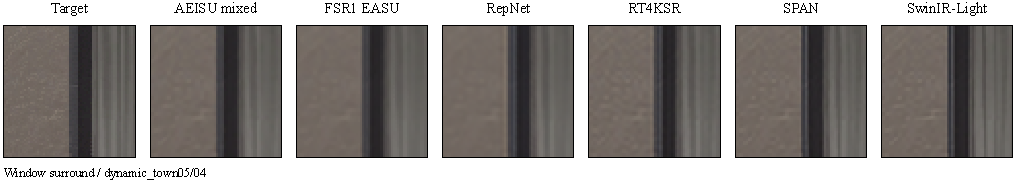
\includegraphics[width=0.85\textwidth]{figures/final_gameir_window_panel.pdf}
\captionof{figure}{\textbf{Additional GameIR edge comparison.} Window surround from GameIR Town05, dynamic sequence 04, frame 00000030, target-derived area input and matched $64\times64$ HR crops. Original colors and nearest-neighbor enlargement. Methods and precision match the main figure. GameIR imagery derives from CARLA assets; attribution and license notices accompany the figures.}
\label{fig:qualitative}
\par
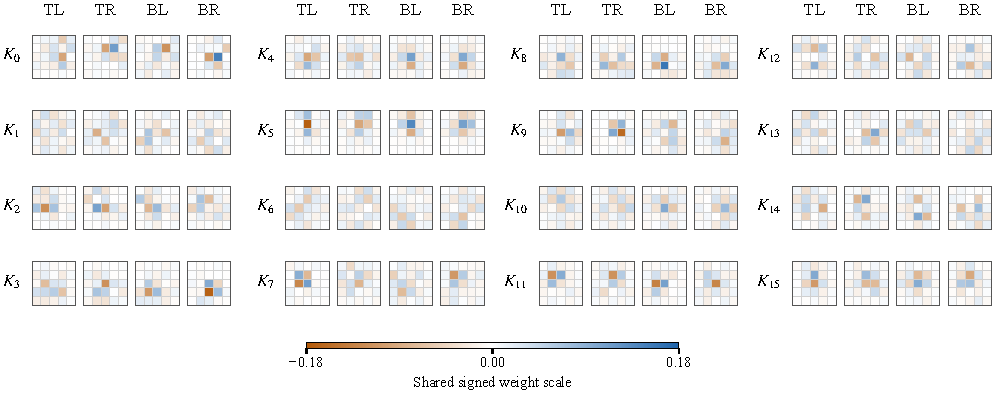
\includegraphics[width=0.85\textwidth]{figures/adaptive_bank_compact.pdf}
\captionof{figure}{\textbf{Learned reconstruction bank.} Sixteen components with four $5\times5$ phases (TL, TR, BL, BR). Each row contains four components. Zero DC, $\ell_1$ norm at most $0.5$, common color range $[-0.18,0.18]$.}
\label{fig:kernels}
\par
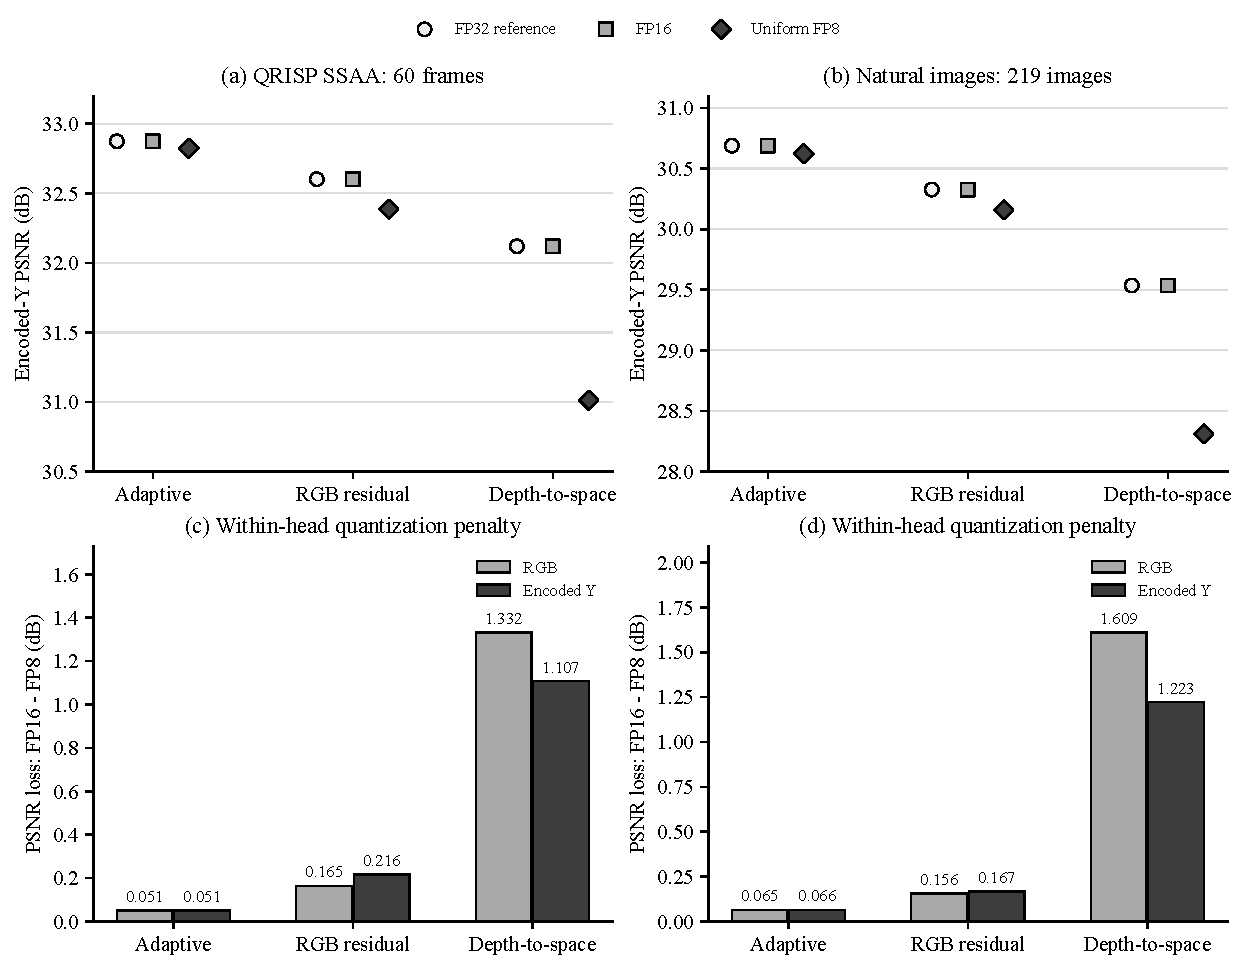
\includegraphics[width=0.58\textwidth]{figures/output_head_quantization_quality.pdf}
\captionof{figure}{\textbf{Output-head precision response.} Top: target Y PSNR for FP32, FP16 and uniform FP8 on 60 QRISP frames and 219 natural images, using the main head-study protocol. Bottom: within-model RGB and Y PSNR loss from FP16 to FP8.}
\label{fig:head-quality}
\end{minipage}\par
\endgroup
}]
\end{document}
